\chapter{Twitter filtering and classification}

\section{Downloading Tweets}

Downloading historical tweets through the official Twitter API is not possible without paying for the enterprise edition\cite{Twitter_api}. Also, most third party tools to download historical tweets are expensive to use. Fortunately there is one free library built for this, and this paper utilised GetOldTweets-python by Jefferson-Henrique\cite{getoldtweets}. Henrique automates Twitter's in-browser search function's scroll loader through JSON calls. The disadvantage of this method is that it only does one handle at a time.

This paper has limited the news agencies to fifteen of the major world-wide English agencies. All have been active on Twitter since at least 2011. The details of these are in Table~\ref{tab:news_agencies}.

These fifteen news agencies tweeted a total of 387,063 tweets in the 18 months from 1st January 2017 to 30th June 2018. For consistency, this paper will refer to them collectively as news tweets, and when referring to specific tweets, will use the Twitter handle.

In the same time period, there were 470 tweets signalling earthquakes from the @USGSted Twitter handle, the official U.S. Geological Survey earthquake alerts. These will be called USGS tweets.

\begin {table}[H]
\caption{News Agencies Used} \label{tab:news_agencies} 
\begin{center}
    \begin{tabu}{||l l l||} 
        \hline
        \rowfont[c]{\bfseries} Agency & Handle & Since \\
        \hline\hline
        Agence France-Presse & @AFP & 2011-09-01 \\
        \hline
        Asian News International & @ANI & 2011-08-01 \\
        \hline
        Associated Press & @AssociatedPress & 2009-06-01 \\
        \hline
        Australian Associated Press & @AAPNewswire & 2011-01-01 \\
        \hline
        Bloomberg & @Bloomberg & 2010-01-01 \\
        \hline
        Canadian Press & @CdnPress & 2009-05-01 \\
        \hline
        Catalan News & @catalannews & 2010-01-01 \\
        \hline
        CNN News & @CNN & 2007-02-01 \\
        \hline
        Dow Jones & @DowJones & 2010-06-01 \\
        \hline
        EFE Noticias & @efenoticias & 2010-01-01 \\
        \hline
        Press Association & @PA & 2009-02-01 \\
        \hline
        Press Trust of India & @PTI\_News & 2011-02-01 \\
        \hline
        Reuters & @Reuters & 2007-03-01 \\
        \hline
        United Press International & @UPI & 2008-10-01 \\
        \hline
    \end{tabu}
\end{center}
\source{Bloomberg\cite{bloomberg}}
\end{table}

\pagebreak
\section{USGS Tweets}

The USGS tweets are in a standardised format. This makes extracting the location, magnitude and time-stamp of the earthquake a simple exercise in string comprehension, as per the code in Listing~\ref{lst:extracting}:

\begin{figure}[H]
\caption{Tweet from USGS on May 9}  \label{fig:USGSTed} 
\centering

\includegraphics[width=0.8\textwidth]{Figures/USGSTed_May9.PNG}
\source{\url{https://Twitter.com/USGSted}}
\end{figure}

The geopy library takes a location string and places it on the globe\cite{geopy}. There are a variety of geocoders to chose from such as Bing Maps, Nominatim and Google. GoogleV3 is the same database driving google maps and provides accurate latitude and longitude, based on a location string entered.

\begin{lstlisting}[caption={Extracting data from standardised USGS tweets}, captionpos=t, label={lst:extracting}]

import numpy as np
from datetime import datetime as dt
from geopy.geocoders import GoogleV3
geolocator = GoogleV3(api_key=private_api_key)
class TweetText():
    #extract magnitude, location and time from standardised tweets by USGSted
    # "Prelim M6.5 earthquake Java, Indonesia Dec-15 16:47 UTC, updates https:// go.usa.gov/xnnuP , 398 #gempa tweets/min"
    def __init__(self, text, date):
        # find the dash from the end of the string
        dash_loc = text[::-1].find('-')
        self.region = text[23:-(dash_loc+4)].strip()
        try:
            location = geolocator.geocode(self.region)
            self.coordinates = (location.latitude, location.longitude)
        except:
            self.coordinates = np.NaN
        self.magnitude = text[8:12].strip()
        self.timestamp = dt.strptime(date[0:4]+'-'+text[-(dash_loc+4):-(dash_loc-8)].strip(), '%Y-%b-%d %H:%M')
        self.details = [self.magnitude, self.region, self.coordinates, self.timestamp]
\end{lstlisting}

The time of earthquake given by USGS is in Coordinated Universal Time (UTC). However, the time-stamp for tweets downloaded from the Twitter website using GetOldTweets is the user's local time. Because, in this case, that is Hong Kong, these times had to be converted to UTC. After conversion, all times in this paper are in 24-hour UTC unless otherwise specified.

The 470 USGS tweets were all processed and cleaned in this way.

\pagebreak
\section{Pre-processing}

\subsection{Network Inputs}

The purpose of this system is to test if a tweet is referring to the same earthquake event as one specified by a USGS tweet. To identify these tweets, a combination of automated filtering and neural network classification will be used. The purpose of the filtering and classification will be to help reduce the amount of work the neural network has to perform, by reducing the inputs to only those most important to classification.

Given that it's possible for two earthquakes to strike in different parts of the world at a similar time, the first input was based on distance. By comparing distances, it will increase the chance of only selecting relevant tweets.

Given the speed that news can travel, it is important to consider the timeliness of the tweets from news agencies. The second input was based on the difference in time between the USGS tweet and the news tweet.

For financial signals, it's important to be first. So as well as the distance and time differences, whether the same news agency, or any news agency has mentioned the tweet or not was also used. Without these checks, multiple tweets from the same source could be identified as relevant.

In summary, the network inputs chosen were:
\begin{itemize}
    \item Great Circle Distance between the earthquake location and the location mentioned in the news tweet
    \item Time from news tweet to USGS tweet
    \item Whether this particular news agency has reported this earthquake before.
    \item Whether any news agency has reported it before.
\end{itemize}

Across the tweets selected, the first two continuous-scale inputs had a correlation of only 0.165 which indicates that it is not likely to have any redundancy from them. By ensuring the number of inputs is contained to the minimum required for a human to check, the complexity of the model is contained.

\subsection{Data Cleansing and Filtering}

A large part of training a neural network is ensuring the data is clean and in a usable form\cite{LeCun_backprop}. There were five steps to this process:

\begin{enumerate}
    \item Filter the data by keyword
    \item Extract locations from the text, translate to coordinates
    \item Merge USGS tweets DataFrame with News Agency tweets DataFrame
    \item Calculate differences between locations and time-stamps
    \item Filter out news agency tweets which happened before the earthquake, or more than three days after the respective USGS tweet.
\end{enumerate}

After all these steps were complete, the manual coding of the data could begin.

The first step in preparing the news agency tweet data was filtering the tweets which also contained key words related to earthquakes. Merriam Webster dictionary highlighted this list related to earthquakes: [`quake', `earthquake', `magnitude', `earthquake', `Richter', `aftershock', `tremor', `seismic', `epicenter', `epicentre']\cite{MerriamWebster2009}.

This left a list of only 1040 tweets, to use in training the neural network. The vast majority were related to earthquakes, such as ``7.9 earthquake strikes near Papua New Guinea, Solomon Islands http:// upi.com/6484906 pic.Twitter.com/j2NjsjAshF" or ``An earthquake of 6.1 magnitude hit Northern and Central Iran at 3.11 am." Unfortunately, some of the tweets were unrelated: ``A `youthquake' struck 2017 as Oxford Dictionaries' word of the year http:// u.afp.com/4Fgx" and ``If the U.N. sexual abuse crisis has an epicenter, it is the Congo.". These tweets were kept and used in training the network. They were classified as unrelated to any earthquake, and will be used by the system to avoid future possible scenarios.

Next, the Polyglot library was used to do named entity recognition for locations of the earthquake the tweets are referring to\cite{polyglotner}. Polyglot was chosen over other NER libraries because it supports languages other than English. In future work it will be important to source tweets from a more global base. The only entities used in this research were locations, using the `I-LOC' tag, as per Listing~\ref{lst:ner}:

\begin{lstlisting}[caption={Named Entity Extraction with polyglot}, captionpos=t, label={lst:ner}]
import polyglot
from polyglot.text import Text
def get_location(blob):
    text = Text(blob, hint_language_code='en')
    location = ''
    for entity in text.entities:
        if entity.tag == 'I-LOC':
            location+= " ".join(entity) + ', '
    return location

df_quakes['location'] =  df_quakes.text.apply(lambda x: get_location(x))

\end{lstlisting}

The 470 USGS tweets were merged to the 1040 tweets to give a DataFrame with 488,800 rows.  The tweets are all time-stamped for publication date which can be used to calculate the time difference between the USGS tweet and the news tweet.

Using the location coordinates indicated in the news tweets and the USGS tweets, the great circle distance between the two points is calculated. Dyck's implementation of the Haversine formula was used\cite{haversine}.

The penultimate step was using the time differences. The time-stamps were converted in the same way as the USGS tweets then rows were removed where:

\begin{enumerate}
    \item the news tweet came before the earthquake time-stamp in the USGS tweet.
    \item the news tweet was more than three days after the USGS tweet
\end{enumerate}

It is important to include news tweets that came before the USGS tweet to test for any news agencies that might have a source faster than USGS, as long as they were after than the actual earthquake. When this final filtering step was complete, there were 3654 rows.

\subsection{Output Coding}

For training, the related tweets need to be manually classified. In classifying, the focus was on Breaking news. Updates on rescue efforts and death toll numbers were considered unrelated as they are no longer useful for identifying an earthquake has occurred.

Figure~\ref{fig:USGSTed} showed an example of the standardised tweets produced by the USGS. It was tweeted at 10:58 on 2018-05-09, and is referring to an earthquake that occurred 17 minutes previously in the Afghanistan-Tajikistan-Pakistan region. Table~\ref{tab:sample_tweets} shows the filtered news tweets within three days of that USGS tweet. 

The first tweet from @ANI that referred to the earthquake was at 11:13, 15 minutes after the USGS tweet, and 32 minutes after the earthquake hit. A number of tweets around that time were marked as not related because they referred to an earthquake that happened in China on the same day, ten years prior. @AFP made two tweets shortly after the earthquake. One at 11:15, that references USGS as a source. They posted again at 13:30, with a story and link. This was quite a common occurrence in the data set. News agencies would post the headline in an attempt to break the news first, and then write a story around it.

Table~\ref{tab:delayed_coverage} shows the average delay after the USGS tweet to the first relevant news agency tweet.

\begin {table}[H]
\caption{How soon do news agencies cover earthquakes?} \label{tab:delayed_coverage}
\begin{center}
    \begin{tabu}{| l r |} 
        \hline
        Shortest Delay: & 3 mins \\
        Mean Delay & 124 mins \\\
        Median Delay & 35 mins \\
        Longest Delay & 977 mins  \\ \hline
    \end{tabu}
\end{center}
\end{table}

\begin{sidewaystable}[htbp]
    \caption{Tweets tested against USGS May 9$^{th}$ tweet}
    \label{tab:sample_tweets}
    \bigskip
    \centering\small\setlength\tabcolsep{2pt}
        \hspace*{-2cm}\begin{tabular}{ p{4cm} p{2cm} p{16cm} p{3cm} }
            \toprule
            \textbf{Tweet Timestamp} & \textbf{Agency} & \textbf{Tweet Text} & \textbf{Classification} \\
            \midrule
2018-05-09 11:13 &  ANI & Earthquake of magnitude 6.2 hit Afghanistan-Tajikistan-Pakistan region: USGS, light tremors were felt in parts of northern India, including Delhi \& Kashmir. & TRUE \\
2018-05-09 11:15 &  AFP & \#BREAKING Strong 6.2-magnitude earthquake rocks Afghanistan: USGS & TRUE \\
2018-05-09 12:00 &  AFP & VIDEO: As China prepares to mark 10 years since the 7.9-magnitude Sichuan earthquake, around 200 people work to preserve the ruined buildings of Beichuan, a city frozen in time since May 12, 2008 pic.Twitter.com/jFd0Y8AW92 & FALSE \\
2018-05-09 13:30 &  AFP & \#UPDATE A strong 6.2-magnitude earthquake has rocked northern Afghanistan, the US Geological Survey says, creating tremors felt as far away as Pakistan's capital Islamabad and Tajikistan's Dushanbe http://u.afp.com/ox8v pic.Twitter.com/RQtx8L7Kb7 & TRUE \\
2018-05-09 14:11 &  CNN & Hawaii residents could face acid rain after earthquakes and molten lava https://cnn.it/2G03r2G pic.Twitter.com/9SZWwYwPXs & FALSE \\
2018-05-09 17:17 &  UPI & Earthquakes strike Afghanistan, Pakistan https://www.upi.com/Top\_News/US/20 18/05/09/ Earthquakes-strike-Afghanistan-Pakistan/1571525883573/?utm\_source=dlvr.it\&utm\_medium=Twitter & TRUE \\
2018-05-09 18:25 &  CNN & Hawaii residents could face acid rain after earthquakes and molten lava https://cnn.it/2rv69be pic.Twitter.com/7EsLzI6utN & FALSE \\
2018-05-10 05:46 &  CNN & Hawaii residents could face acid rain after earthquakes and molten lava https://cnn.it/2rygcw5 pic.Twitter.com/7rp3vm2S47 & FALSE \\
2018-05-10 06:28 &  AFP & Life among the ruins: Chinese village 10 years after devastating earthquake in Sichuan left 87,000 people dead or missing http://u.afp.com/oxbq Johannes Eisele @johaynz pic.Twitter.com/CENCPfllNP & FALSE \\
2018-05-10 07:52 &  AFP & VIDEO: 'Strong Pig' is a celebrity in China after surviving the devastating Sichuan earthquake a decade ago that left 87,000 people dead or missing pic.Twitter.com/Iap71OHFR5 & FALSE \\
2018-05-10 09:22 &  CNN & Hawaii residents could face acid rain after earthquakes and molten lava https://cnn.it/2KRrm7Z pic.Twitter.com/grKq4ruf3A & FALSE \\
2018-05-10 19:42 &  AFP & VIDEO: The tiny hamlet of Radish Village in China's southwest is one of several in Sichuan province that decided to preserve the destruction as a memorial to the 2008 earthquake pic.Twitter.com/7FwXCEqPQE & FALSE \\
2018-05-11 18:02 &  Reuters & Hawaii residents shaken by quakes, brace for new lava outbreaks https://reut.rs/2rBJ0UG & FALSE \\
2018-05-11 20:16 &  Reuters & Hawaii residents shaken by tremors, brace for new lava outbreaks https://reut.rs/2KS5kSG & FALSE \\
2018-05-12 07:06 &  UPI & On This Day: Sichuan earthquake kills tens of thousands https://www.upi.com/Top\_News/2018/ 05/12/On-This-Day-Sichuan-earthquake-kills-tens-of-thousands/4111526048817/ ?utm\_source=dlvr.it\&utm\_medium=Twitter & FALSE \\
2018-05-12 07:31 &  ANI & An earthquake of magnitude 3.0 on the Richter scale hit Chamba region of \#HimachalPradesh at 9:27 am today & FALSE \\
           \bottomrule
        \end{tabular}
        \source{Twitter }
        \hspace*{-2cm}
\end{sidewaystable}

Of the 3654 records in the training data only 294, or 8\% were coded as relating the news tweet to an earthquake.

\begin{figure}[H]
\centering
 \caption{Tweet Classification Summary}
 \label{fig:classification}
\begin{tikzpicture}
 \pie [rotate = 0]
    {8/ Related tweets,
     92/ Not-related tweets}
\end{tikzpicture}
\end{figure}

\subsection{Dividing the Data Set}

As discussed in Sub-section~\ref{subsubsec:fitting} the data needs to be divided into three sets; training, validation and testing.

75\% of the data set was randomlly selected to be used as training, and 25\% to be used as testing. The next step is to divide the training set into the actual training data and the validation data set. A similar algorithm was used to assign 20\% of the training data to a validation set. The final breakdown can be seen in table~\ref{tab:breakdown}.

\begin {table}[H]
\caption{Data set Breakdown} \label{tab:breakdown}
\begin{center}
    \begin{tabu}{| c c c c | } 
        \hline
        \rowfont[c]{\bfseries} Data Set & Records & \% of Total & \% Related \\
        \hline\hline
        Training Set & 2192 & 60 & 8.0 \\
        Validation Set & 548 & 15 & 7.1 \\
        Testing Set & 914 & 25 & 8.6 \\ \hline
        \textbf{Total} & \textbf{3654} & \textbf{100} & \textbf{8.0}\\ \hline
    \end{tabu}
\end{center}
\end{table}

While running training iterations, this was repeated for each iteration, as well as randomising the initial weights. As mentioned in Sub-section\ref{subsec:weights} Keras automatically randomises the initial weights according to Glorot's algorithm\cite{chollet2015keras}.

\pagebreak
\section{ANN Setup}

There are a large number of freely available machine learning resources for python. This streamlines the model building process. This project utilises a high-level neural network API called Keras\cite{chollet2015keras} running on top of Google's the TensorFlow framework\cite{tensorflow2015-whitepaper}.

\subsection{Normalisation Layer}

Before attempting to train a network with this data, it is important to normalise the inputs, as discussed in Chapter 2's section on normalisation (\ref{normalisation}). For the distance and time inputs, the min-max method was used. All distances were represented as a percentage of the maximum possible distance (half the earth's circumference). All times were converted to seconds, and calculated as a percentage of the seconds in three days: $3 * 24 * 60 * 60 = 259 200$, including the negative values. The tests on whether or not a particular news agency covered an earthquake before was coded from True/False to 1/0.

\subsection{Network Topology Set-up}

As discussed, there are four normalised inputs to the neural network. In all cases for this network, boolean data is represented by 0 for False, and 1 for True.
\begin{itemize}
  \item Great Circle Distance: as a percentage of the earth’s half circumference
  \item Time Lapsed: as a percentage of 3 days
  \item Whether this news agency has reported it: boolean
  \item Whether any news agency has reported it: boolean
\end{itemize}

If any of these fields are not useful in calculating the outputs, their weights will tend towards zero. The output, expected of the neural network is whether or not it is related to the earthquake.

\begin{figure}[H]
\caption{Example of the neural network}
\centering
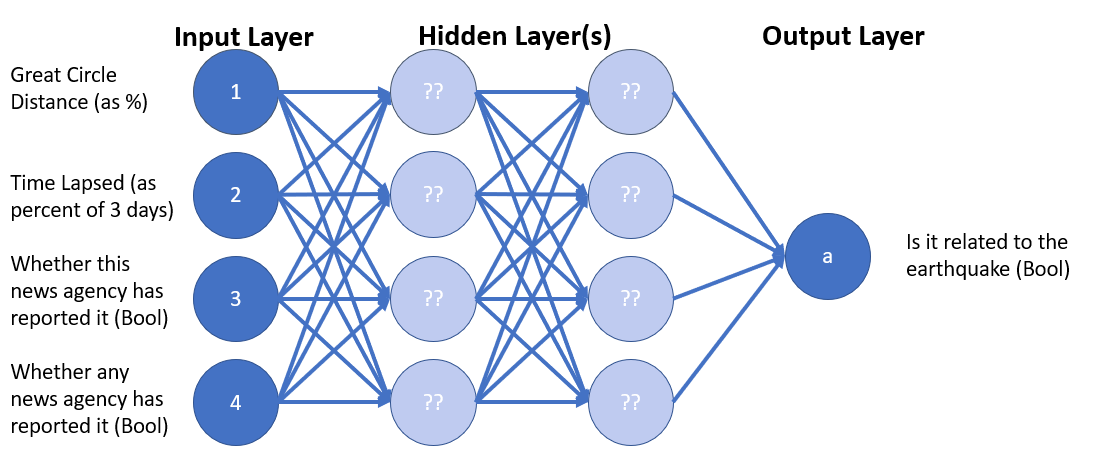
\includegraphics[width=1.0\textwidth]{Figures/SampleNetwork.PNG}
\end{figure}

For such a simple data set, a deep network will likely not be required. Prior research\cite{LeCun_backprop}\cite{Goodfellow_deeplearning}\cite{huang_two_layer} suggests one or two-layers will be sufficient.

Reviewing formulas ~\ref{eq:first_layer} and ~\ref{eq:second_layer} in Chapter 2, the number of outputs, $m$ is 1, the number of training samples, $N$, is 2192.
\begin{align*}
    1^{st} \text{Layer}&= \sqrt{\left(m+2\right)N} + 2\sqrt{N/\left(m+2\right)} \\
    &= \sqrt{\left(1+2\right)2192} + 2\sqrt{2192/\left(1+2\right)} \\
    &= 135 \\
    2^{nd} \text{Layer}&= m\sqrt{N/\left(m+2\right)} \\
    &= 1\sqrt{2192/\left(1+2\right)} \\
    &= 27  
\end{align*}

This narrows our search space for the topology but still leaves a large space to search for a two-layer network. There were a number of rules-of-thumb described in Chapter 2, regarding topology setup. In terms of limiting the space, one of these suggested that each layer should be no more than twice the number of inputs to that layer. This would limit the size of the first layer to 8 neurons.

\subsection{Network Topology Optimisation}

As discussed in sub-section~\ref{subsubsec:topology}, there is no golden rule for deciding on the best neural network topology. After finding boundaries for the space, the simplest models were tested with a list of initial learning rates. If insufficient results were not obtained following the rules-of-thumb, more nodes can be added.

The initial weights, if selected poorly could cause the model to reach a local, but not global minimum. To avoid the random weights causing a particular topology to be excluded because of this, all topologies were tested five times with the same random weights. This was managed by seeding the random number generator in Keras, which implements the uniform distribution range suggested by Glorot\cite{Glorot_difficulties}.

Because this is a classification-style problem, the output layer was tested with both the sigmoid and tanh activation functions. The hidden layers were tested with ReLU and leaky ReLU (with different $\alpha$ values).

\begin{lstlisting}[caption={Initial Space Search}, captionpos=t, label={lst:initial_search}]
lrs=[0.01, 0.05, 0.1]
first= 10
second= 10
for lr in lrs:
    for f in range(1,first):
        for s in range(0,second):
            for i in range(5):
                #compile model with random weights, seed i
                
                #fit model with training and validation data
                
                #evaluate model on test data
            # save best model for (lr,f,s)
\end{lstlisting}

When s is zero, in the inner most loop, it signals a single layer network, and the second hidden layer is not added.

The more complex models ($f+s > 10$) were observed to perform very well on training sets, but poorly on the test set validation. This is an indication that they were over-fitting the data. This is consistent with the rules of thumb outlined in sub-section~\ref{subsubsec:topology}.

\pagebreak
\section{Training}

Training of a neural network requires the fine-tuning of hyper-parameters to find the combination that not only learns from the training set, but is general enough to perform well on an unseen test set.

To speed up training, and avoid over-fitting, an Early Stopping callback was implemented. This callback checked the loss function on the validation data set every epoch. If it had not improved by at least 0.1\%, within the last 10 epochs, the model was considered trained and the next area of the space was searched.

The maximum epochs was set to 200. However, because of the early stopping callback, most training runs stopped learning after 50-80 epochs.

Binary cross-entropy was used as the loss function, as discussed in sub-section~\ref{subsubsec:loss_func}. Binary accuracy was also measured as a metric. As discussed in Sub-section~\ref{subsubsec:loss_func}, this is best-practise for classification problems where the output is True/False. Keras has already implemented these functions.

When a suitably small initial search space was identified, from analysing the results of the topology search, further analysis was conducted with various learning rates and momentum rates:

\begin{align*}
    lrs &= [0.14, 0.1, 0.05, 0.02, 0.01, 0.005, 0.001, 0.0001, 0.00001]  \\
    mrs &= [0.0, 0.5, 0.6, 0.7, 0.8, 0.9]
\end{align*}

This follows the values suggested in subsection~\ref{subsubsec:hyperparams}. The models were judged on their loss function when applied to the test set. The model with the smallest loss function on the test set was deemed to be the best model, and predictions from that model were used in calculating the threshold for categories.

\section{Prediction Threshold}

In order to achieve the highest rate of precision, while minimising the type 1 and type 2 errors of the predictions, different thresholds were examined. Using the two kinds of ROC graphs, the AOCs can be calculated and compared.

Firstly, using the traditional ROC test. The tp rate and np rates were calculated for each 1\% increment from 0\% to 100\%. True predictions for every value above the threshold, False predictions for every value below the threshold. From this the AUC for each was calculated and the largest AUC gave the optimal result.

Similarly, for the adjusted ROC test, when un-defined is allowed as a response. The tp rate and np rates were calculated for each 1\% increment away from 50\%. True predictions for every value greater than $50+x\%$ and false predictions for every value less than $50-x\%$, with the undefined band in the middle. Again, the AUC for each was calculated and the largest AUC gave the optimal result.


%When writing the Methods section  must clearly identify the statistical methods  will use to generate the results needed to meet the research objectives and the research scope.
%²  must also demonstrate that  understand all assumptions associated with the methods  used and justify why those methods are appropriate for your research.
%² For example,  cannot just state \Bootstrapping methods will be used to generate con¯dence intervals for the population correlation coe±cient."  need to show that your study meets the necessary assumptions to use bootstrapping methods to generate con¯dence intervals for the population correlation coe±cient.
%² Remember that `methods' are di®erent than `results'. Therefore,  should not be presenting summaries (such as tables and ¯gures of results) in the Methods chapter. 
%Do cannot assume that your committee members or anyone who will read the dissertation understands the methods  used. Therefore, in the Methods chapter,  should Clearly describe the methods.  should provide enough details so that anyone %reading the dissertation would know how to replicate your research.
%Justify why the statistical methods are appropriate.
%Include simple examples that demonstrate an application of methods.